% !TEX TS-program = pdflatex
% !TEX encoding = UTF-8 Unicode

% This is a simple template for a LaTeX document using the "article" class.
% See "book", "report", "letter" for other types of document.

\documentclass[11pt]{article} % use larger type; default would be 10pt

\usepackage[utf8]{inputenc} % set input encoding (not needed with XeLaTeX)

%%% Examples of Article customizations
% These packages are optional, depending whether you want the features they provide.
% See the LaTeX Companion or other references for full information.

%%% PAGE DIMENSIONS
\usepackage{geometry} % to change the page dimensions
\geometry{a4paper} % or letterpaper (US) or a5paper or....
% \geometry{margin=2in} % for example, change the margins to 2 inches all round
% \geometry{landscape} % set up the page for landscape
%   read geometry.pdf for detailed page layout information

\usepackage{graphicx} % support the \includegraphics command and options

% \usepackage[parfill]{parskip} % Activate to begin paragraphs with an empty line rather than an indent

%%% PACKAGES
\usepackage{booktabs} % for much better looking tables
\usepackage{array} % for better arrays (eg matrices) in maths
\usepackage{paralist} % very flexible & customisable lists (eg. enumerate/itemize, etc.)
\usepackage{verbatim} % adds environment for commenting out blocks of text & for better verbatim
\usepackage{subfig} % make it possible to include more than one captioned figure/table in a single float
% These packages are all incorporated in the memoir class to one degree or another...

%%% HEADERS & FOOTERS
\usepackage{fancyhdr} % This should be set AFTER setting up the page geometry
\pagestyle{fancy} % options: empty , plain , fancy
\renewcommand{\headrulewidth}{0pt} % customise the layout...
\lhead{}\chead{}\rhead{}
\lfoot{}\cfoot{\thepage}\rfoot{}

%%% SECTION TITLE APPEARANCE
\usepackage{sectsty}
\allsectionsfont{\sffamily\mdseries\upshape} % (See the fntguide.pdf for font help)
% (This matches ConTeXt defaults)

%%% ToC (table of contents) APPEARANCE
\usepackage[nottoc,notlof,notlot]{tocbibind} % Put the bibliography in the ToC
\usepackage[titles,subfigure]{tocloft} % Alter the style of the Table of Contents
\renewcommand{\cftsecfont}{\rmfamily\mdseries\upshape}
\renewcommand{\cftsecpagefont}{\rmfamily\mdseries\upshape} % No bold!

%%% END Article customizations



\usepackage[table]{xcolor}
\usepackage{geometry}
\usepackage{pdflscape}

%%% The "real" document content comes below...

\title{Translating a Classifier}
\author{Patrick Martin}
%\date{} % Activate to display a given date or no date (if empty),
         % otherwise the current date is printed 

\begin{document}
\maketitle

\section{Overview}



\subsection{The Data}

In order to work on translating a classifier, I need similar data in different languages. The first thing I'm going to use is reddit, starting with March 2017 (and adding others if I need more data), using langdetect (https://pypi.python.org/pypi/langdetect) on comments that have at least 15 unique words. I'm going to try to pull 10k each of Spanish, French, and Italian. Unfortunately this is either slow or sparse, and is taking a while. Hopefully it will finish by tomorrow or something.

Alternatively/additionally, if I can find different-language wikipediae, I can use page category as the classes.

\subsubsection{LID data}

We can make sure the LID worked reasonably well by checking the subreddits represented


\rowcolors{2}{gray!25}{white}
\begin{tabular}{l|c}
\rowcolor{gray!50} Subreddit & Count  \\
argentina & 4,632 \\
mexico & 1,840 \\
podemos\footnote{Spanish political party} & 1,622 \\
chile & 592 \\
vzla & 280 \\
Argaming & 87 \\
Spanish & 80 \\
uruguay & 75 \\
PuertoRico & 50 \\
Colombia & 44 \\

\end{tabular}
\footnotetext[1]{Spanish political party}
\begin{tabular}{l|c}
\rowcolor{gray!50} Subreddit & Count  \\
france & 7,772 \\
Quebec & 1,052 \\
montreal & 197 \\
ParisComments & 116 \\
French & 44 \\
Lyon  & 35 \\
FiascoQc & 34 \\
SquaredCircle\_FR & 32 \\
effondrement & 27 \\
melenchon & 23 
\end{tabular}
\begin{tabular}{l|c}
\rowcolor{gray!50} Subreddit & Count  \\
italy & 7,862 \\
oknotizie & 525 \\
ItalyInformatica & 351 \\
italy\_SS & 327 \\
italygames & 86 \\
perlediritaly & 69 \\
lisolachece & 62 \\
Romania & 61 \\
ItaliaPersonalFinance & 54 \\
ItalyMotori & 40
\end{tabular}

\subsubsection{Subreddit corpora}

Using the data from the LID stuff, we can also just create the corpora by using all the posts from some subreddits. I propose\footnote{We'll fix this later} \\

\begin{tabular}{c}
\rowcolor{gray!50} Spanish  \\
argentina \\
mexico \\
chile \\
vzla \\
uruguay \\
Colombia \\
\end{tabular}
\begin{tabular}{c}
\rowcolor{gray!50} French  \\
france \\
Quebec \\
montreal \\
Lyon  \\
\end{tabular}
\begin{tabular}{c}
\rowcolor{gray!50} Italian  \\
italy \\
\end{tabular}

\section{Classifier}

In order to make this work, we need to have some aspect that we're trying to classify against. One thing that has been done in the past is classification based on subreddit; based on the subreddits represented this could be possible: national subreddit (argentina, france, italy), gaming (Argaming, jeuxvideo, italygames), however maybe not much else. For reference, these are the fields I have to work with for each comment: \\

\begin{tabular}{c c c c c} 
author & author\_flair\_css\_class & author\_flair\_text & body & controversiality \\
created\_utc & distinguished & edited & gilded & id \\
 link\_id & parent\_id & retrieved\_on & score & stickied \\
 subreddit & subreddit\_id \end{tabular}

Here are what I think:
\begin{itemize}
\item Controversiality \\
\emph{Pro:} Should be fairly language independent \\
\emph{Con:} Pretty sparse, only about 3\% of the documents are ``controversial''. Controversial comments might tend to be in English, as well (comments from outsiders)

\item Score: (binned) \\
\emph{Pro:} Should be fairly language independent \\
\emph{Con:} Borderlines between bins might be difficult, also more extreme scores are very sparse ($<$ 0.2\% have scores of at least 100)

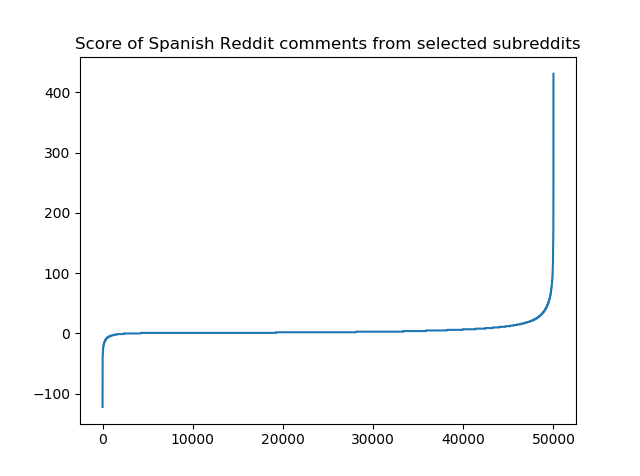
\includegraphics[scale=0.5]{spanish_score.png}

\item Gilded: (binary) \\
\emph{Pro:} Should be fairly language independent \\
\emph{Con:} Extremely sparse ( < 0.03\% have been gilded)

\item Subreddit: \\
\emph{Pro:} Definitely influenced by context \\
\emph{Con:} Might be biased either towards games that are available in the given language, or the text will involve a lot of English.

\item Flair (submissions): \\
\emph{Pro:} Human-decided topic labels
\emph{Con:} Submissions are not as common as comments, and the flairs across different subreddits might not align perfectly. Additionally, the title might not represent the content of the link perfectly.
\end{itemize}

The last idea just sort of came to me while looking at the subreddits. Using title text of submissions might be a good side project if this turns promising. To be specific, this is the number of comments in the smallest class for each of \emph{gilded}, \emph{controversial}, and \emph{score}. (For \emph{gilded} and \emph{controversial}, this is the number of positive examples). \\

\begin{tabular}{|c|c|c|c|}
& Gilded&Contro &Score \\
Spanish-sub & 3& 347& 123\\
Spanish & 0& 52& 16\\
French-sub & 1& 423& 70\\
French & 0 & 64& 10\\
Italian-sub & 1& 189& 24\\
Italian & 1& 59& 15\\
\end{tabular}

First, it's pretty clear that gilded isn't going to work well at all. Second, the bins for score might need to be refined.

\section{Initial Classifiers}

I divided my data into 80\% train and 20\% test and ran a couple classifiers on all of the data. Since \emph{score} is multi-class, the default F1 score doesn't make sense, all of these classifiers will be evaluated on the harmonic mean of the fscores for each class\footnote{Is this a real thing?}. I'm not sure if this is actually something that's really used, but it will work for our comparison purposes.

\begin{tabular}{|c|c|c|c|}
\rowcolor{gray!50}\multicolumn{4}{|c|}{naive bayes} \\
& Gilded&Contro&Score \\
Spanish-sub & 0.0100& 0.0001& 0.0002\\
Spanish & 1.0000& 0.0007& 0.0013\\
French-sub & 0.0392& 0.0185& 0.0002\\
French & err& 0.0006& 0.0004\\
Italian-sub & 0.0392& 0.0002& 0.0004\\
Italian & 0.0392& 0.0006& 0.0011\\
\end{tabular}
\quad \rowcolors{2}{gray!25}{white}
\begin{tabular}{|c|c|c|c|}
\rowcolor{gray!50}\multicolumn{4}{|c|}{logistic regression} \\
& Gilded&Contro&Score \\
Spanish-sub & 0.0100& 0.1551& 0.1145\\
Spanish & err& 0.0004& 0.1513\\
French-sub & 0.0198& 0.1889& 0.0644\\
French & err& 0.1523& 0.0079\\
Italian-sub & 0.0392& 0.1902& 0.0038\\
Italian & err& 0.1198& 0.0057\\
\end{tabular}



\section{Bootstrapping}
Recalling that controversial comments make up about 3\% of the documents, and that classifiers are remarkably bad at picking them out, could we maybe train up a classifier to pick them out by bootstrapping? First, a look at the data:\\
\begin{tabular}{|c|c|c|c|}
\rowcolor{gray!50} & \# Documents & \# Controversial & \% \\
Spanish & 163,057 & 5,243 & 3.2\% \\
French & 207,348 & 9,449 & 4.6\% \\
Italian & 79,479 & 3,048 & 3.8\% \end{tabular}\\


We're going to look at Spanish first. Here is the (initial) algorithm:

\begin{enumerate}
\item Pick 5,000 documents at random (Random init)
\item Train some classifiers on those documents, splitting the 5,000 into random 80\% train and 20\% test sets (NOTE: these are not the same for each classifier)
We'll use Naive Bayes (NB) and Logistic Regression (LR), run three different times. The table will show the one that works best
\item Pick the classifier with the best f-score, and run it over all the documents
\item Pick the 5,000 documents rated most likely to be controversial by that classifier, excluding any documents previously seen
\item Repeat
\end{enumerate}

%\begin{tabular}{|c|c|c|l|l|l|l|}
%\rowcolor{gray!50} &&& \multicolumn{4}{|c|}{Classifier f-score} \\
%\rowcolor{gray!50} & Doc count & \# Yes & NB1\footnotemark & NB2 & LR1\footnotemark & LR2 \\
%Random init & 5000 & 140 & 0 & 0 & 0 & \textbf{0.18} \\
%Round 1 & 9983 & 451 (+311) & 0 & 0 & 0.079 & \textbf{0.086} \\
%Round 2 & 14983 & 720 (+269) & 0 & 0 & \textbf{0.097} & 0.085 \\
%Round 3 & 19983 & 970 (+250) & 0 & 0 & 0.11 & 0.14 \\
%\end{tabular}
\begin{tabular}{|c|l|l|l|l|l|}
\rowcolor{gray!50} &&&& \multicolumn{2}{|c|}{Classifier f-score} \\
\rowcolor{gray!50} & Doc count & \# Yes (repeats) & \# Yes (total) & NB & LR \\
Random init & 5000 & 172 (3.4\%)& 172 & 0 & \textbf{0.087} \\
Round 1 & 5000 & 399 (8.0\%) & 437 (+265)& 0 & \textbf{0.077} \\
Round 2 & 5000 & 574 (11.5\%) & 683 (+246) & 0 & \textbf{0.16} \\
Round 3 & 5000 & 710 (14.2\%) & 928 (+245) & 0 & \textbf{0.097} \\
\end{tabular}
\\
Some initial takeaways are that Naive Bayes just can't learn in this environment, but otherwise this process does work. Let's modify the algorithm to see if we can't make Naive Bayes a little happier:

\begin{enumerate}
\item Pick 5,000 documents at random (Random init)
\item Train some classifiers on \emph{a subset of the documents, making sure positive documents comprise 33\% of the dataset}, splitting \emph{it}	 into random 80\% train and 20\% test sets (NOTE: these are not the same for each classifier)
We'll use Naive Bayes (NB) and Logistic Regression (LR), run three different times. The table will show the one that works best
\item Pick the classifier with the best f-score, and run it over all the documents
\item Pick the 5,000 documents rated most likely to be controversial by that classifier, excluding any documents previously seen
\item Repeat
\end{enumerate}
\begin{tabular}{|c|l|l|l|l|l|}
\rowcolor{gray!50} &&&& \multicolumn{2}{|c|}{Classifier f-score} \\
\rowcolor{gray!50} & Doc count & \# Yes (repeats) & \# Yes (total) & NB & LR \\
Random init & 5000 & 173 (3.5\%) & 173 & \textbf{0.16} & 0.30 \\
Round 1 & 5000 & 381 (7.6\%) & 429 (+256) & \textbf{0.36} & 0.43 \\
Round 2 & 5000 & 553 (11.1\%) & 702 (+273) & \textbf{0.31} & 0.40 \\
Round 3 & 5000 & 724 (14.5\%) & 1000 (+298) & \textbf{0.38}  & 0.47
\end{tabular}
\\
Indeed, this did help Naive Bayes get on the scoreboard. Both it and LR improved drastically, although LR still remained ahead. For this batch I decided to bootstrap based on the best NB classifier, to see if it bootstrapped well. Indeed, the general results are very similar. How does this work for French?

\begin{tabular}{|c|l|l|l|l|l|}
\multicolumn{6}{|c|}{Without subsetting} \\
\rowcolor{gray!50} &&&& \multicolumn{2}{|c|}{Classifier f-score} \\
\rowcolor{gray!50} & Doc count & \# Yes (repeats) & \# Yes (total) & NB & LR \\
Random init & 5000 & 216 (4.3\%) & 216 & 0 & \textbf{0.10} \\
Round 1 & 5000 &  571 (11.4\%) & 621 (+405)& 0.017 & \textbf{0.12} \\
Round 2 & 5000 & 883 (17.7\%) & 1034 (+413)& 0 & \textbf{0.17} \\
Round 3 & 5000 & 1124 (22.5\%) & 1432 (+398) & 0.0067 & \textbf{0.16} \\
\end{tabular}
\\
\begin{tabular}{|c|l|l|l|l|l|}
\multicolumn{6}{|c|}{With subsetting} \\
\rowcolor{gray!50} &&&& \multicolumn{2}{|c|}{Classifier f-score} \\
\rowcolor{gray!50} & Doc count & \# Yes (repeats) & \# Yes (total) & NB & LR \\
Random init & 5000 & 243 (4.9\%) & 243 & \textbf{0.42} & 0.49 \\
Round 1 & 5000 & 533 (10.7\%) & 637 (+394)& \textbf{0.35} & 0.44 \\
Round 2 & 5000 & 828 (16.6\%) & 1095 (+458)& \textbf{0.36} & 0.44 \\
Round 3 & 5000 & 1041 (20.8\%) & 1523 (+428)& \textbf{0.38} & 0.44 \\
\end{tabular}

Looks like it works very similarly, with a bonus probably because French has more controversial posts.

\subsection{Pruning with Logistic Regression}

On the pruning experiments, I purposely chose to snowball the Naive Bayes to make sure it actually worked. However, Logistic Regression still had better F-scores, and so it's worth seeing how it does: \\

\begin{tabular}{|c|l|l|l|l|l|}
\multicolumn{6}{|c|}{Spanish} \\
\rowcolor{gray!50} &&&& \multicolumn{2}{|c|}{Classifier f-score} \\
\rowcolor{gray!50} & Doc count & \# Yes (repeats) & \# Yes (total) & NB & LR \\
Random init & 5000 & 170 & 170 & 0.24 & 0.49 \\
Round 1 & 5000 & 397 & 460 (+291) & 0.29 & 0.42 \\
Round 2 & 5000 & 577 & 732 (+272) & 0.38 & 0.38 \\
Round 3 & 5000 & 745 & 1029 (+297) & 0.25 & 0.42 \\
\end{tabular} \\
\begin{tabular}{|c|l|l|l|l|l|}
\multicolumn{6}{|c|}{French} \\
\rowcolor{gray!50} &&&& \multicolumn{2}{|c|}{Classifier f-score} \\
\rowcolor{gray!50} & Doc count & \# Yes (repeats) & \# Yes (total) & NB & LR \\
Random init & 5000 & 226 & 226 & 0.23 & 0.34 \\
Round 1 & 5000 & 434 & 572 & 0.21 & 0.46 \\
Round 2 & 5000 & 772 & 992 & 0.24 & 0.35 \\
Round 3 & 5000 & 1026 & 1413 & 0.28 & 0.44 \\
\end{tabular}


\subsection{SVM}

\begin{tabular}{|c|l|l|l|l|}
\multicolumn{5}{|c|}{Without subsetting} \\
\rowcolor{gray!50} &&& \multicolumn{2}{|c|}{Classifier f-score} \\
\rowcolor{gray!50} & Doc count & \# Yes (repeats) & \# Yes (total) & SVM \\
Translated init & 5000 & 151 (3.0\%) & 151 & 0.03 \\
Round 1 & 5000 &  297 (6.0\%) & 329 & 0.06 \\
Round 2 & 5000 & 423 (8.5\%) & 492 & 0.04 \\
Round 3 & 5000 & 593 (11.9\%) & 705 & 0.05 \\
\end{tabular} \quad

\begin{tabular}{|c|l|l|l|l}
\multicolumn{5}{|c|}{With subsetting} \\
\rowcolor{gray!50} &&& \multicolumn{2}{|c|}{Classifier f-score} \\
\rowcolor{gray!50} & Doc count & \# Yes (repeats) & \# Yes (total) & SVM \\
Translated init & 5000 & 168 (3.4\%) & 168 & 0.39 \\
Round 1 & 5000 & 272 (5.4\%) & 438 & 0.38 \\
Round 2 & 5000 & 264 (5.3\%) & 702 & 0.42 \\
Round 3 & 5000 & 247 (4.9\%) & 949 & 0.40
\end{tabular} \\

Oh yeah, SVM doesn't give probabilities, so it doesn't really make sense to ask for the 5,000 most likely documents. What if we instead make it so that we use the three SVM classifiers and rank by voting?

\subsection{Many Runs}
For the purposes of the next section, we're going to need a classifier that works reasonably well. Let's snowball the hell out of this thing. \\

\begin{tabular}{|c|*{6}{l|}}
\rowcolor{gray!50} & Doc count & \# Yes (repeats) & \# (total) & NB & LR & SVM \\
Random init & 5000 & 178 (3.6\%) & 178 & 0 & 0.4 & \emph{0.05} \\
Round 1 & 5000 & 331 (6.6\%) & 365 & 0 & \emph{0.12} & 0.07 \\
Round 2 & 5000 & 535 (10.7\%) & 621 & 0 & \emph{0.09} & 0.06 \\
Round 3 & 5000 & 723 (14.5\%) & 915 & 0 & \emph{0.12} & 0.10 \\
Round 4 & 5000 & 845 (16.9\%) & 1191 & 0 & \emph{0.14}& 0.13\\
Round 5 & 5000 & 1051 (21.0\%) & 1429 & 0 & \emph{0.14} & 0.11\\
Round 6 & 5000 & 1258 (25.2\%) & 1692 & 0 & \emph{0.15} & 0.11\\
Round 7 & 5000 & 1462 (29.2\%) & 1912 & 0.01 & \emph{0.15} & 0.12\\
Round 8 & 5000 & 1673 (33.5\%) & 2127 & 0.00 & \emph{0.18} & 0.13\\
Round 9 & 5000 & 1840 (36.8\%) & 2310 & 0.01 & \emph{0.15} & 0.14\\
Round 10 & 5000 & 1977 (39.5\%) & 2528 & 0.01 & \emph{0.15} & 0.13 \\
\end{tabular}
NB never really did so hot, but what if we take that last LR and now do some pruning\\
\begin{tabular}{|c|*{6}{l}}
\rowcolor{gray!50} & Doc count & \# Yes (repeats) & \# (total) & NB & LR & SVM \\
Round 1 & 5000 & 2178 & 2713 & 0.33 & \emph{0.45} & 0.45 \\
Round 2 & 5000 & 1534 & 2956 & 0.30 & \emph{0.45} & 0.43 \\
Round 3 & 5000 & 1556 & 3197 & 0.35 & \emph{0.45} & 0.44 \\
Round 4 & 5000 & 1571 & 3370 & 0.34 & \emph{0.45} & 0.42 \\
Round 5 & 5000 & 1540 & 3542 & 0.34 & \emph{0.46} & 0.42
\end{tabular}


\subsection{Different tokenizer}
Right now it's word tokenization, but what if we changed it to word 2grams? \\

\begin{tabular}{|c|*{6}{l|}}
\rowcolor{gray!50} & Doc count & \# Yes (repeats) & \# (total) & NB & LR & SVM \\
Random init & 5000 & 156  & 156 & 0 & 0.13 & 0.11 \\
Round 1 & 5000 & 364 & 403 & 0 & 0.07 & 0.04 \\
Round 2 & 5000 & 570 & 683 & 0.02 & 0.16 & 0.18 \\
Round 3 & 5000 & 713 & 841 & 0.01 & 0.11 & 0.12 \\
Round 4 & 5000 & 892 & 1116 & 0.01 & 0.11 & 0.08 \\
Round 5 & 5000 & 973 & 1338 & 0.01 & 0.12 & 0.13 \\
\end{tabular}


\section{Translating a Classifier}
The reason we used word tokenization for the classifiers on the bootstrapping, and why we wanted Naive Bayes to work well, is that we're going to try to translate a classifier that works on Spanish to one that works on French. To start, we have a heavily bootstrapped (Round 9) that, in Spanish, has 1,542 of its 5,000 (30.8\%) best documents as controversial.

Here's the initial plan:
\begin{enumerate}
\item Start with a fairly good classifier (30\% accuracy)
\item Grab 500 words that strongly indicate either `yes' or `no' to controversiality in this classifier (250 from each side) 
\item Translate those words to French
\item Build a new classifier from these words
\item Evaluate the quality
\end{enumerate}

For simplicity, we're just going to use Google Translate to translate the words. Additionally, our first attempt to build the classifier is to use word embeddings trained on the French corpus to infer controversiality based on similarity:

\[ p(class|word) \propto \sum_{w\in N_k(word)} p(class|w) sim(word,w) \]

where $N_k(word)$ represents the $k$-nearest ``anchor'' words, with $k$=5. This gives us probabilities for all 8,554 words that occur at least 100 times. So how does this do?\\

\begin{tabular}{|c|l|l|l|l|l|}
\multicolumn{6}{|c|}{Without subsetting} \\
\rowcolor{gray!50} &&&& \multicolumn{2}{|c|}{Classifier f-score} \\
\rowcolor{gray!50} & Doc count & \# Yes (repeats) & \# Yes (total) & NB & LR \\
Translated init & 5000 & 213 (4.3\%) & 213 & 0 & 0.05 \\
Round 1 & 5000 &  537 (10.7\%) & 599 & 0.03 & 0.09 \\
Round 2 & 5000 &  803 (16.1\%) & 979 & 0 & 0.14 \\
Round 3 & 5000 & 1069 (21.4\%) & 1383 & 0.008 & 0.17 \\
\end{tabular}
\quad
\begin{tabular}{|c|l|l|l|l|l|}
\multicolumn{6}{|c|}{With subsetting} \\
\rowcolor{gray!50} &&&& \multicolumn{2}{|c|}{Classifier f-score} \\
\rowcolor{gray!50} & Doc count & \# Yes (repeats) & \# Yes (total) & NB & LR \\
Random init & 5000 & 213 & 213 & 0.25 & 0.39 \\
Round 1 & 5000 & 298 & 415 & 0.28 & 0.42 \\
Round 2 & 5000 & 620 & 738 & 0.32 & 0.45 \\
Round 3 & 5000 & 764 & 1045 & 0.39 & 0.46 \\
\end{tabular} \\

Remember, this was French, so this does about as well as a random French model. Let's see if we can improve this at all.

\subsection{Spanish to Spanish}

To help improve the algorithm, let's take the translations out of it, and instead just build a new model on Spanish from a good original model. Doing the same process as before, we get \\

\begin{tabular}{|c|l|l|l|l|l|}
\rowcolor{gray!50} &&&& \multicolumn{2}{|c|}{Classifier f-score} \\
\rowcolor{gray!50} & Doc count & \# Yes (repeats) & \# Yes (total) & NB & LR \\
Translated init & 5000 & 150 (3.0\%) & 150 & 0 & 0.09 \\
Round 1 & 5000 &  392 (7.8\%) & 428 & 0 & 0.10 \\
Round 2 & 5000 & 586 (11.7\%)& 689 & 0.01 & 0.11 \\
Round 3 & 5000 & 697 (13.9\%) & 971 & 0 & 0.11
\end{tabular} \\

This is about on par with what we usually get. What if we look at the word embeddings?

\subsubsection{Word Embeddings}

The word embeddings were created using gensim word2vec on the Spanish reddit corpora. Reddit comments are incredibly terrible for NLP tools to work with, namely because
\begin{itemize}
\item Multiple authors \\
\item Informal speech \\
\item Multiple languages (mostly English) \\
\item Short comments\end{itemize}

So, how well is our word embedding doing? Let's check what words it considers "most similar" for some common words

\begin{tabular}{c|c|c|c|c}
\rowcolor{gray!50} nosotros & agua & argentina & hombre & tienda \\
articulos & bariloche & llev\'abamos & denunicados & burocr\'aticas \\ 
pas\'a & peleados & indicado & chaos & comunismo \\
rpgs & paleont\'ologo & odies & uriburu & migratorio \\
enojar & ajusten & curado & cerebral & militan \\
apel\'o & machote & permiten & surprised & luca \end{tabular}

In other words, this is trash. We might ask if it's still useful trash though. For how many words does the controversiality of a word agree with its 5 closest neighbors? Well, first off, the words that get marked as controversial more often than not actually tend to be fairly uncommon words. To be sure:
\\
\begin{tabular}{c|c|c}
\rowcolor{gray!50} & All words & Controversial words \\
\# & 40,483 & 8,369 \\
Average frequency & 11.04 & 2.56 \\
\# with at least 100 occurances & 453 & 3 \\
\# with at least 20 occurances & 2,160 & 103 \\\end{tabular}
\\
So this is another problem with using word embeddings, is that the controversial words are ones whose meaning won't be captured very well. Anyway, as for neighbor agreement, with a cutoff of 20 occurances: \\
\begin{tabular}{c|c|c}
\rowcolor{gray!50} Neighbors agreeing & Controversial & Non-controversial \\
0 & 78 & 0 \\
1 & 25 & 0 \\
2 & 0 & 4 \\
3 & 0 & 69 \\
4 & 0 & 474 \\
5 & 0 & 1480 \end{tabular}\\

In other words, the controversial words don't pick each other out at all. Do they at least pick out maybe more-controversial words? What if we ask what is the combined controversiality ($y/(y+n)$) of the five nearest neighbors, the five furthest neighbors, and five random words?

\begin{tabular}{c|c|c}
\rowcolor{gray!50}\%   & Controversial & Non-controversial \\
Neighbors & 32.1\% &  32.9\%\\
Anti-neighbors & 32.3\% & 32.9\% \\
Average & 32.8\% &  32.8\% \end{tabular}\\

In other words: yes, these word embeddings are complete trash. I found pre-trained word embeddings here: http://crscardellino.me/SBWCE/, which apparently are actually good word embeddings. What happens if we run the previous tests?\\


\begin{tabular}{c|c|c|c|c}
\rowcolor{gray!50} nosotros & agua & argentina & hombre & tienda \\
tenemos & potable & uruguaya & mujer& tiendas \\
nos & potabiliza & Argentina & muchacho & supermercado \\
pensamos & tierra & chilena & joven & zapater\'ia\\
Nosotros & potabilizada & bonaerense & anciano & abarrotes\\
estamos & semisurgente & argentinas & gavillero & autoservicio \\
\end{tabular} \\

Alright, that's a good sign. How about controversiality now?\\

\begin{tabular}{c|c|c}
\rowcolor{gray!50} Neighbors agreeing & Controversial & Non-controversial \\
0 & 56 & 0 \\
1 & 21 & 0 \\
2 & 8 & 14 \\
3 & 6 & 62 \\
4 & 0 & 373 \\
5 & 0 &1552 \end{tabular}\\

\begin{tabular}{c|c|c}
\rowcolor{gray!50}\%   & Controversial & Non-controversial \\
Neighbors & 34.3\% &  31.3\%\\
Anti-neighbors & 31.0\% & 30.0\% \\
Average & 32.8\% &  32.8\% \end{tabular}\\

So yeah, it looks like having better word embeddings does actually help a little. However, it's still not that distinguishing.

\subsection{Getting more controversial words}

One problem appears to be that we don't have good data on controversial words. To counteract this, let's just train the Naive Bayes on \emph{all} of the data, so that it has controversial counts on every word. 


\subsection{Translating Logistic Regression}

Logistic regression is just the discriminative version of Naive Bayes, so it should lend itself to this task fairly nicely too. However, that's not the case, as doing this gives \\

\begin{tabular}{|c|*{6}{l|}}
\rowcolor{gray!50} & Doc count & \# Yes (repeats) & \# (total) & NB & LR & SVM \\
Translated init & 5000 & 123 (2.5\%) & 123 & 0 &  0.15 & 0.09 \\
Round 1 & 5000 &  276 (6.1\%) & 304 &  0 & 0.13 & 0.04 \\
Round 2 & 5000 & 463 (9.3\%)& 530 & 0.02 & 0.10 & 0.07 \\
Round 3 & 5000 & 600 (12.0\%) & 812 & 0 & 0.14 & 0.10 \\
\end{tabular} \\
If we restrict the words to need to occur at least 100 times in order to be considered for translation, we get

\begin{tabular}{|c|*{6}{l|}}
\rowcolor{gray!50} & Doc count & \# Yes (repeats) & \# (total) & NB & LR & SVM \\
Translated init & 5000 & 224 (4.5\%) & 224 & 0 & 0.14 & 0.10 \\
Round 1 & 5000 &  461 (9.2\%) & 504 & 0.02 & 0.10 & 0.08 \\
Round 2 & 5000 &  652 (13.0\%) & 785 & 0.01 & 0.11 & 0.11 \\
Round 3 & 5000 &  819 (16.4\%) & 1044 & 0 & 0.16 & 0.10 \\
\end{tabular} \\
Hey, now that's not too bad. As a reminder, with a random initialization, we start with about 3.2\% controversial and end with about 14\%, so we've improved over the baseline by about 10\%. 


\section{To-Do}
Here's what's currently left to do:
\begin{itemize}
\item Evaluate Spanish to Spanish ``translation''
\item Produce images of Spanish word embeddings with colors for controversiality (do same for French)
\item Implement Logistic Regression translation
\item Implement Topic Model similarity
\item Get new word embeddings
\item Look at 2-gram word embeddings
\end{itemize}

\end{document}
